This part is to identify voltage-frequency response of ZX95-850+ voltage controlled oscillator. \\

\begin{figure}[h]
\centering
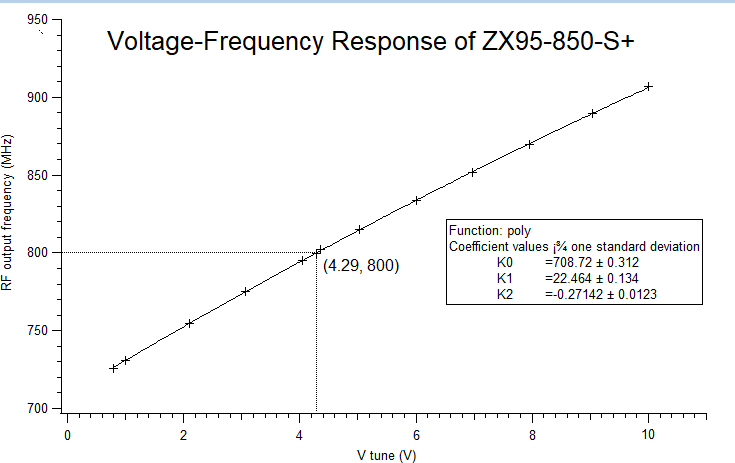
\includegraphics[width=0.8\textwidth]{figures/partA1.png}
\caption{Voltage-frequency response of ZX95-850-S+. The error in measurements was too small to be displayed in the graph. ($\pm 0.01MHz$)}
\end{figure}
The voltage-frequency response of the VCO is shown above. It is close to a linear graph, but it is a parabolic graph with the best fit equation below:
\begin{equation}
    Frequency(MHz)=-0.27142V_{tune}^{2}+22.464V_{tune}+708.72
\end{equation}
With above equation, $f=800MHz$ when $V_{tune}\cong 4.29V$. To determine the slope at 800MHz, we just differentiated above equation and substituted $V_{tune}\cong 4.29V$.
\begin{equation}
    slope(800MHz) = -0.54284V_{tune}+22.464=(20.135 \pm 0.922)MHz/V
\end{equation}

Error anaysis
\begin{equation}
    \Delta slope=slope\cdot \sqrt{(\frac{0.0246}{0.54280})^{2}+(\frac{0.134}{22.464})^{2}+(\frac{0.01}{4.29})^{2}}=0.922
\end{equation}

\subsection{Additional Questions}
1.Comparison with the known data from the Minicircuits web-site. The equation of the parabolic best fit function is :
\begin{figure}[h]
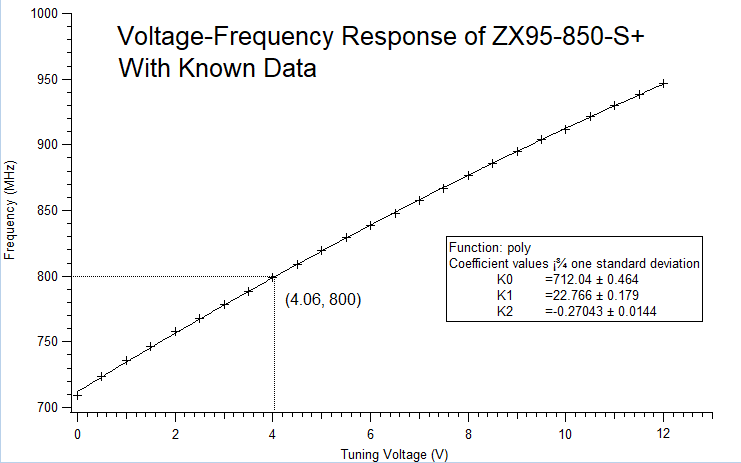
\includegraphics[width=0.8\textwidth]{figures/partA2.png}
\caption{Voltage-frequency response of ZX95-850-S+ when T=25'C with given data from the Minicircuits web-site. }
\end{figure}

\begin{equation}
    Frequency(MHz)=-0.27043V_{tune}^{2}+22.766V_{tune}+712.04 \label{V2F}
\end{equation}
Substituting $f=800MHz,$ $V_{tune}\cong 4.06V$. The slope with the differentiated equation is:
\begin{equation}
    slope(800MHz)=-0.54086V_{tune}+22.766=(20.570 \pm 1.108)MHz/V
\end{equation}

Error analysis
\begin{equation}
        \Delta slope=slope\cdot \sqrt{(\frac{0.0288}{0.54086})^{2}+(\frac{0.179}{22.766})^{2}+(\frac{0.01}{4.06})^{2}}=1.108
\end{equation}

\begin{equation}
    \frac{slope_{known}-slope_{measured}}{slope_{known}}=0.021
\end{equation}
\begin{equation}
    \left | \frac{V_{800MHz}^{known}-V_{800MHz}^{measured}}{V_{800MHz}^{known}} \right |=\left | \frac{4.06-4.29}{4.06} \right |\cong 5.7 percents
\end{equation}
The slope at $f=800MHz$ of the known data is only 2.1 percents off from the slope of the measured data, and they agree to each other within the error range calculated. 
The constants of parabolic best fits agrees to each other within ~1 percents of error. 
The difference between $V_{tune}$ values when $f=800MHz$ is 5.7 percents which is higher than others, but this is due to the voltage drawn from the extra components of the circuit (ie. wire). The extra voltage drawn caused x-shift in right direction of the graph, but it did not affect on the slope when the frequency is 800MHz. \\
There should be an error due to the temperature of the laboratory. Although the temperature was not explicitly measured, it was lower than 25'c, which is the temperature that the known data collected. However, change in voltage-frequency response of VCO due to the temperature is neglible. In Minicircuits website, data collected with T=-55'C and T=85'C have no mentionable difference with data with T=25'C. Therefore, error due to the temperature can be ignored.

2.The isolator is an equipment that transmits radio frequency in one direction only. In this circuit the isolator is used to reduce phase noise of the VCO.